\documentclass{report}

% Packages nécessaires
\usepackage[utf8]{inputenc}
\usepackage[T1]{fontenc}
\usepackage[french]{babel}
\usepackage{titlesec}
\usepackage{tocloft}
\usepackage{lipsum} % Package de remplissage de texte (à retirer dans le rapport final)
\usepackage{graphicx}
\usepackage{float} % pour l'option de placement [H]
\usepackage[colorlinks=true, linkcolor=blue, citecolor=green]{hyperref}
\usepackage{minted} % pour la coloration syntaxique
\usepackage{lipsum}
\usepackage{wrapfig}   % Pour l'enroulement du texte autour des images
\usepackage{array}

% Mathématiques
\usepackage{amsmath, amssymb}
\usepackage{amsthm}
\usepackage{mdframed}  % Package pour les cadres


\newmdtheoremenv{boxedproperty}{Propriété}[section]  % Crée un environnement encadré pour les propriétés


% Configuration de la page
\usepackage[a4paper, left=2.5cm, right=2.5cm, top=2.5cm, bottom=2.5cm]{geometry}

% Pour avoir le petit dessin de l'INSA en bas à droite de chaque page
\usepackage{background}
\backgroundsetup{
scale=1,
angle=0,
opacity=1,
color=black,
contents={\begin{tikzpicture}[remember picture,overlay]
\node at ([xshift=-0.8in,yshift=0.8in] current page.south east) % Adjust the position of the logo.
{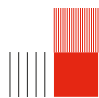
\includegraphics[scale=0.8]{images/pattern.png}}; % logo goes here
\end{tikzpicture}}
}


% Configuration des titres des sections et sous-sections
\titleformat{\chapter}[display]
  {\normalfont\Large\bfseries}{\chaptertitlename\thechapter}{14pt}{}
\titleformat{\section}
  {\normalfont\Large\bfseries}{\thesection}{1em}{}
\titleformat{\subsection}
  {\normalfont\large\bfseries}{\thesubsection}{1em}{}

% Configuration de la table des matières
\renewcommand{\cftchapfont}{\bfseries}
\renewcommand{\cftsecfont}{\normalfont}
\renewcommand{\cftsubsecfont}{\normalfont}
\renewcommand{\cftchappagefont}{\bfseries}
\renewcommand{\cftsecpagefont}{\normalfont}
\renewcommand{\cftsubsecpagefont}{\normalfont}
\setlength{\cftbeforetoctitleskip}{0pt}
\setlength{\cftaftertoctitleskip}{10pt}
\renewcommand{\contentsname}{Table des matières}



\begin{document}


% Page de titre
\begin{titlepage}
    \centering

    % Minipages pour les logos
    \noindent % Assure qu'il n'y a pas d'indentation au début de la ligne
    \begin{minipage}{0.5\textwidth}
        
\includegraphics[width=0.5\linewidth]{images/logo_INSA.png} % Ajustez le chemin et la taille
    \end{minipage}%
    \hfill % Assure que les deux minipages seront poussés à l'extrême gauche et droite
    \begin{minipage}{0.5\textwidth}
        \flushright % Alignement à droite dans la minipage
        
\includegraphics[width=0.5\linewidth]{images/blanc.jpg} % Ajustez le chemin et la taille
    \end{minipage}


    \vspace*{2cm} % Espace vertical de 2 cm
    {\Huge\bfseries Optimisation et parallelisation OpenMP d'addition et produit
de deux matrices denses \par}
    \vspace{1cm}
    {\huge Rapport de Burreau d'étude\par}
    \vspace{2cm}
    {\Large \textbf{Luc-Christelle Nguyen et Alicia Perrin} \par}
    \vspace{2cm}
    
    {\Large \textbf{Institut National des Sciences Appliquées de Toulouse} \par}
    \vspace{1cm}
    {\large \today \par}
\end{titlepage}

% Résumé concis, souvent utilisé pour donner un aperçu rapide du contenu d'une recherche ou d'un article académique.
\begin{abstract}
    Dans ce rapport, nous présenterons différentes méthodes d’optimisation et de parallélisation appliquées aux calculs sur des matrices denses. Nous commencerons par étudier l’impact de l’ordre d’accès à la mémoire sur les performances, en exploitant la proximité spatiale des données afin d’améliorer l’utilisation du cache.Nous explorerons ensuite l’utilisation des bibliothèques OpenMP et OpenBLAS dans le but d’accélérer les calculs. L’analyse des trois niveaux de routines BLAS (BLAS1, BLAS2, BLAS3) mettra en évidence les gains considérables que l’on pourra obtenir grâce à OpenBLAS. Nous testerons également différentes stratégies de parallélisation (options static et dynamic) et nous étudierons l’impact du nombre de threads utilisés sur les performances globales. Enfin, nous mettrons en œuvre une optimisation basée sur la division en blocs (cache blocking) afin de mieux exploiter la hiérarchie mémoire.
\end{abstract}

% Table des matières
\tableofcontents

\newpage


\chapter{Modifier l'accès à la mémoire pour additionner deux matrices}

La première optimisation dont nous nous sommes servis utilise la proximité spatiale des informations. Nous avons fait en sorte que, pour l'addition de deux matrices, l'algorithme parcourt d'abord les lignes et ensuite les colonnes. En effet, une matrice est stockée en mémoire ligne par ligne. Lorsque la fonction va aller chercher la première valeur de la matrice, elle va remplir le cache de avec les valeurs suivantes. Ainsi, grâce à une bonne utilisation du cache, un grand nombre d'accès mémoire sont évités, ce qui permet d'augmenter la performance du programme.

\begin{figure}[H]
    \centering
    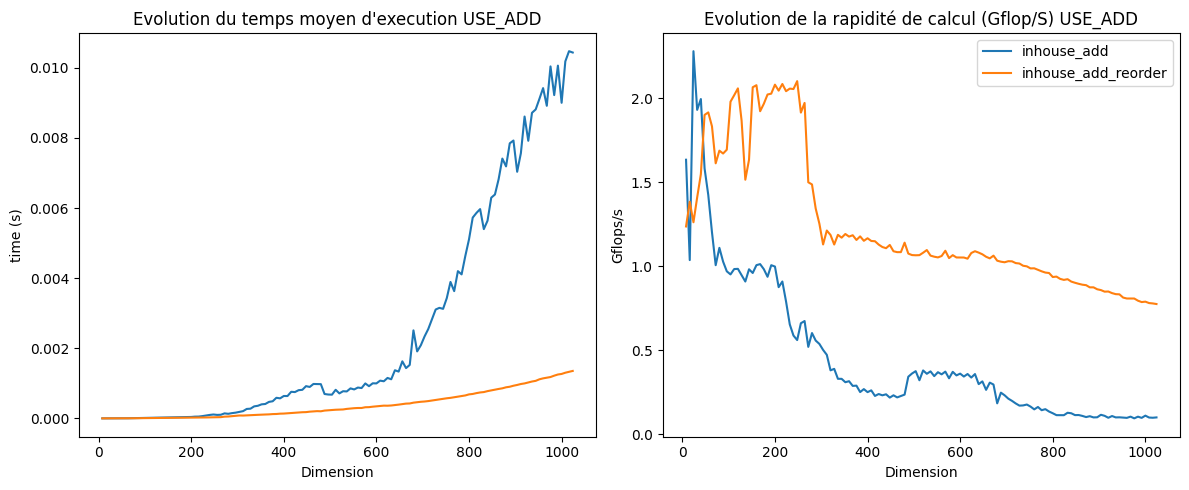
\includegraphics[width=0.7\linewidth]{images/fig3.png}
    \caption{Différences de performances en fonction de l'ordre d'accès à la mémoire}
    \label{fig:3}
\end{figure}


On peut remarquer sur ces simulations que la rapidité de calcul a doublé en moyenne (cf \ref{fig:3}). C'est donc un critère important à prendre en compte lors de l'élaboration d'un programme.


\chapter{Compilation reliant les librairies OpenMP et BLAS}

Il y a trois routines BLAS (Basic Linear Algebra Subprograms) différentes, qui sont des fonctions standards pour effectuer des calculs de base en algèbre linéaire :
\begin{itemize}
    \item BLAS1 : ce sont des opérations vecteur-vecteur. Pour effectuer un produit matrice-matrice en utilisant uniquement des routines BLAS1, il faut appeler la routine pour chaque élément de la matrice résultat (car chaque élément est le produit scalaire d'une ligne et d'une colonne).
    \item BLAS2 : ce sont des opérations matrice-vecteur. Pour calculer un produit matrice-matrice avec des routines BLAS2, il faut appeler la routine pour chaque colonne de la matrice résultat.
    \item BLAS3 : ce sont des opérations matrice-matrice. Un seul appel de la routine permet de calculer tout le produit matriciel.
\end{itemize}


\begin{figure}[H]
    \centering
    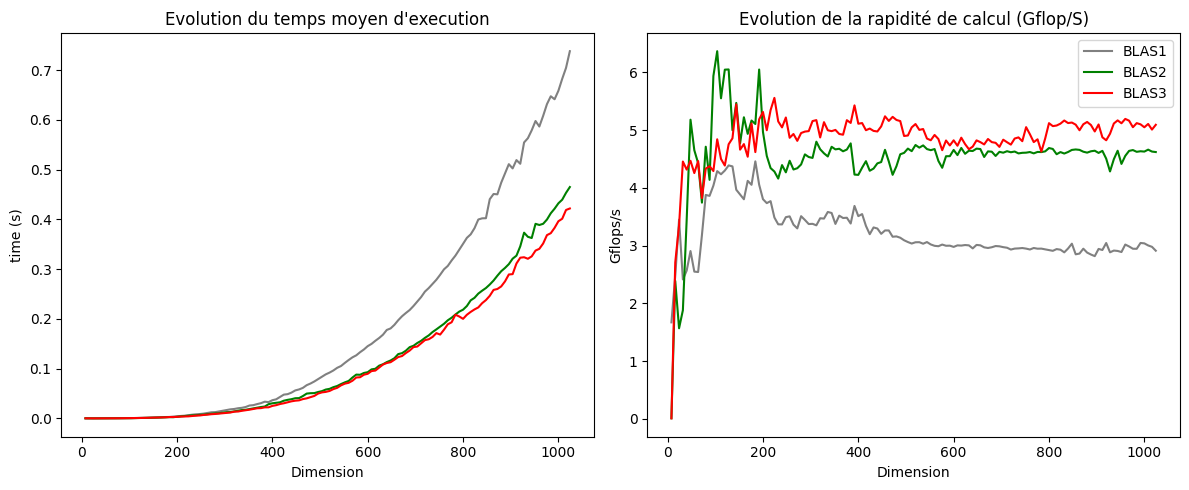
\includegraphics[width=0.7\linewidth]{images/fig1.png}
    \caption{Performances BLAS 1, 2, 3 sans optimisation Openblas}
    \label{fig:1}
\end{figure}

\begin{figure}[H]
    \centering
    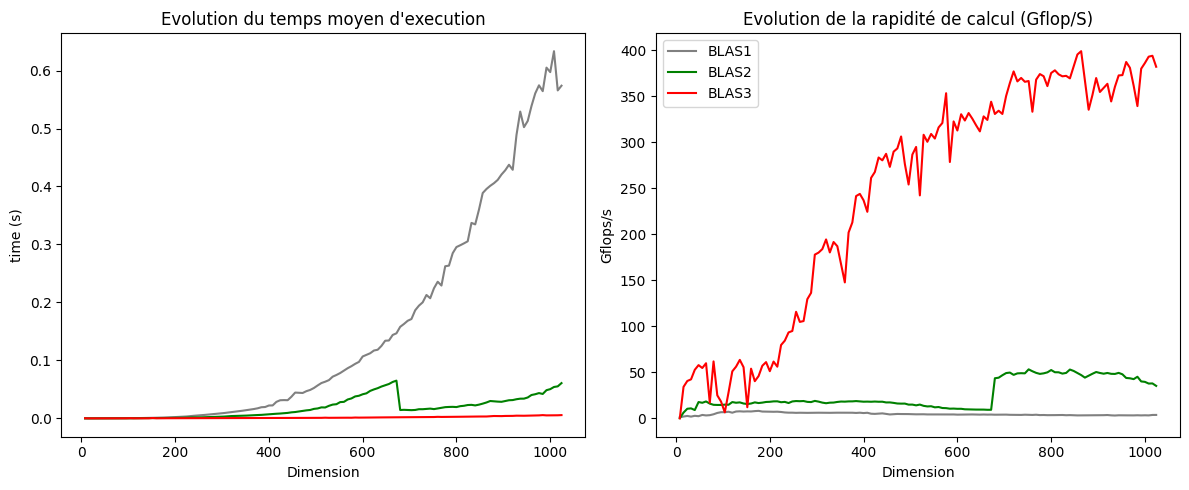
\includegraphics[width=0.7\linewidth]{images/fig2.png}
    \caption{Performances BLAS 1, 2, 3 avec optimisation Openblas}
    \label{fig:2}
\end{figure}

Lors de ces simulations, nous avons voulu premièrement montrer la différence d'efficacité entre les différents BLAS (cf. \ref{fig:1}). On remarque que BLAS3 est légèrement meilleure que les autres, du fait qu'il ne fait appel qu'à une seule fonction.
Puis nous avons voulu montrer la nette amélioration des performances lorsque nous utilisons la librairie OpenBLAS. C'est une version rapide et optimisée des routines BLAS. Elle utilise des optimisations spécifiques au processeur pour exploiter au mieux les instructions vectorielles et le calcul parallèle sur plusieurs cœurs. La différence de performance est énorme. Par exemple, pour BLAS3 la rapidité de calculs passe de 5Gflops à 400Gflops (cf \ref{fig:2}).

\chapter{Options de parallelisation d'un produit matriciel}

Dans cette partie, nous nous sommes concentrées sur l'optimisation par la parallélisation des tâches. Dans les simulations qui suivent, nous avons voulu tester les différentes options de parallélisation.

\begin{figure}[H]
    \centering
    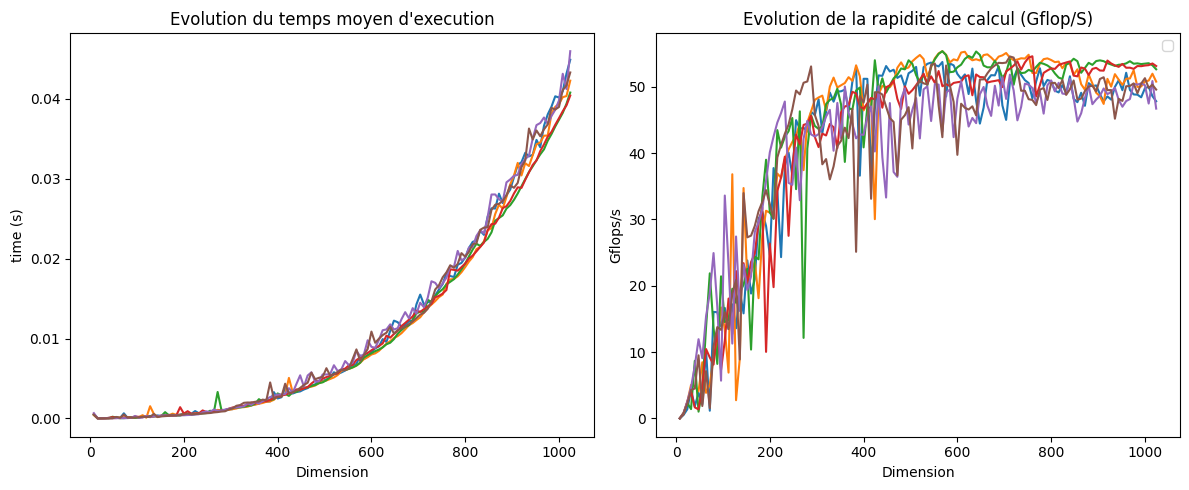
\includegraphics[width=0.7\linewidth]{images/fig4.png}
    \caption{Performances d'un calcul matriciel parallélisé avec l'option static et différents nombres de coeurs disponibles}
    \label{fig:4}
\end{figure}

\begin{figure}[H]
    \centering
    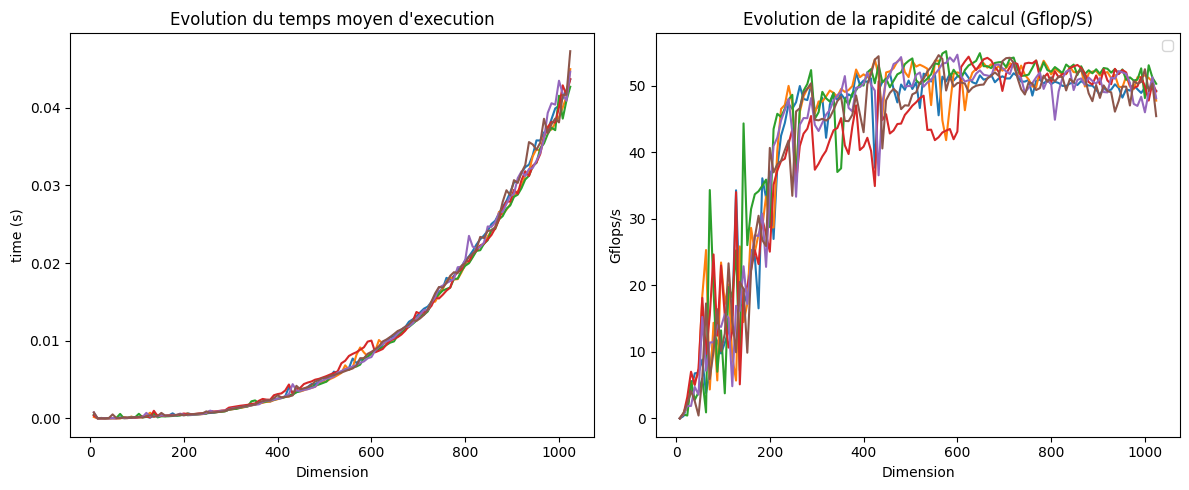
\includegraphics[width=0.7\linewidth]{images/fig5.png}
    \caption{Performances d'un calcul matriciel parallélisé avec l'option dynamic et différents nombres de coeurs disponibles}
    \label{fig:5}
\end{figure}

Nous pouvons remarquer que changer ces options n'a aucune influence réelle sur la performance du programme.

\chapter{Nombre de threads utilisé pour BLAS3}
\begin{figure}[H]
    \centering
    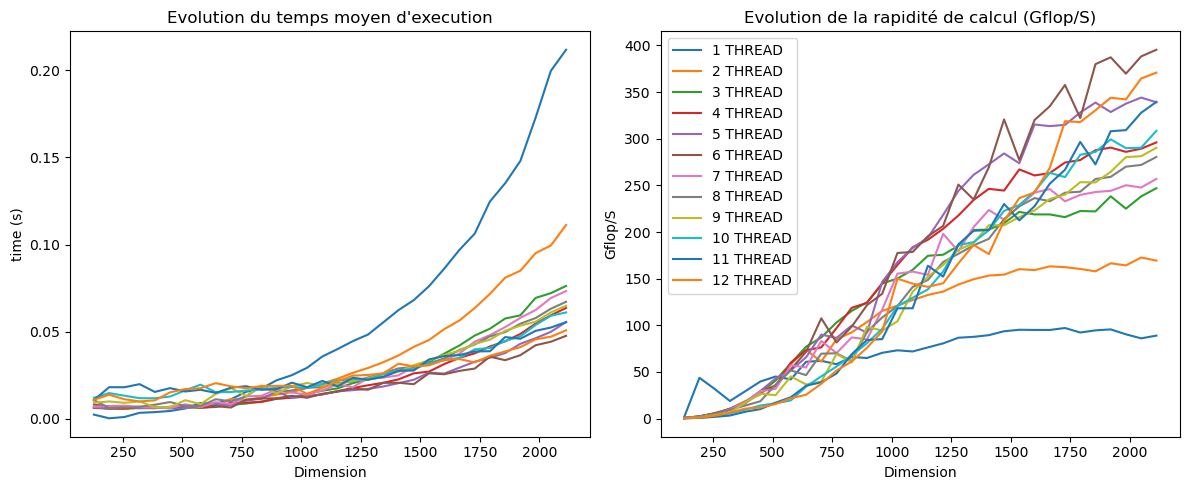
\includegraphics[width=0.7\linewidth]{images/fig6.png}
    \caption{Trouver titre}
    \label{fig:6}
\end{figure}

\begin{figure}[H]
    \centering
    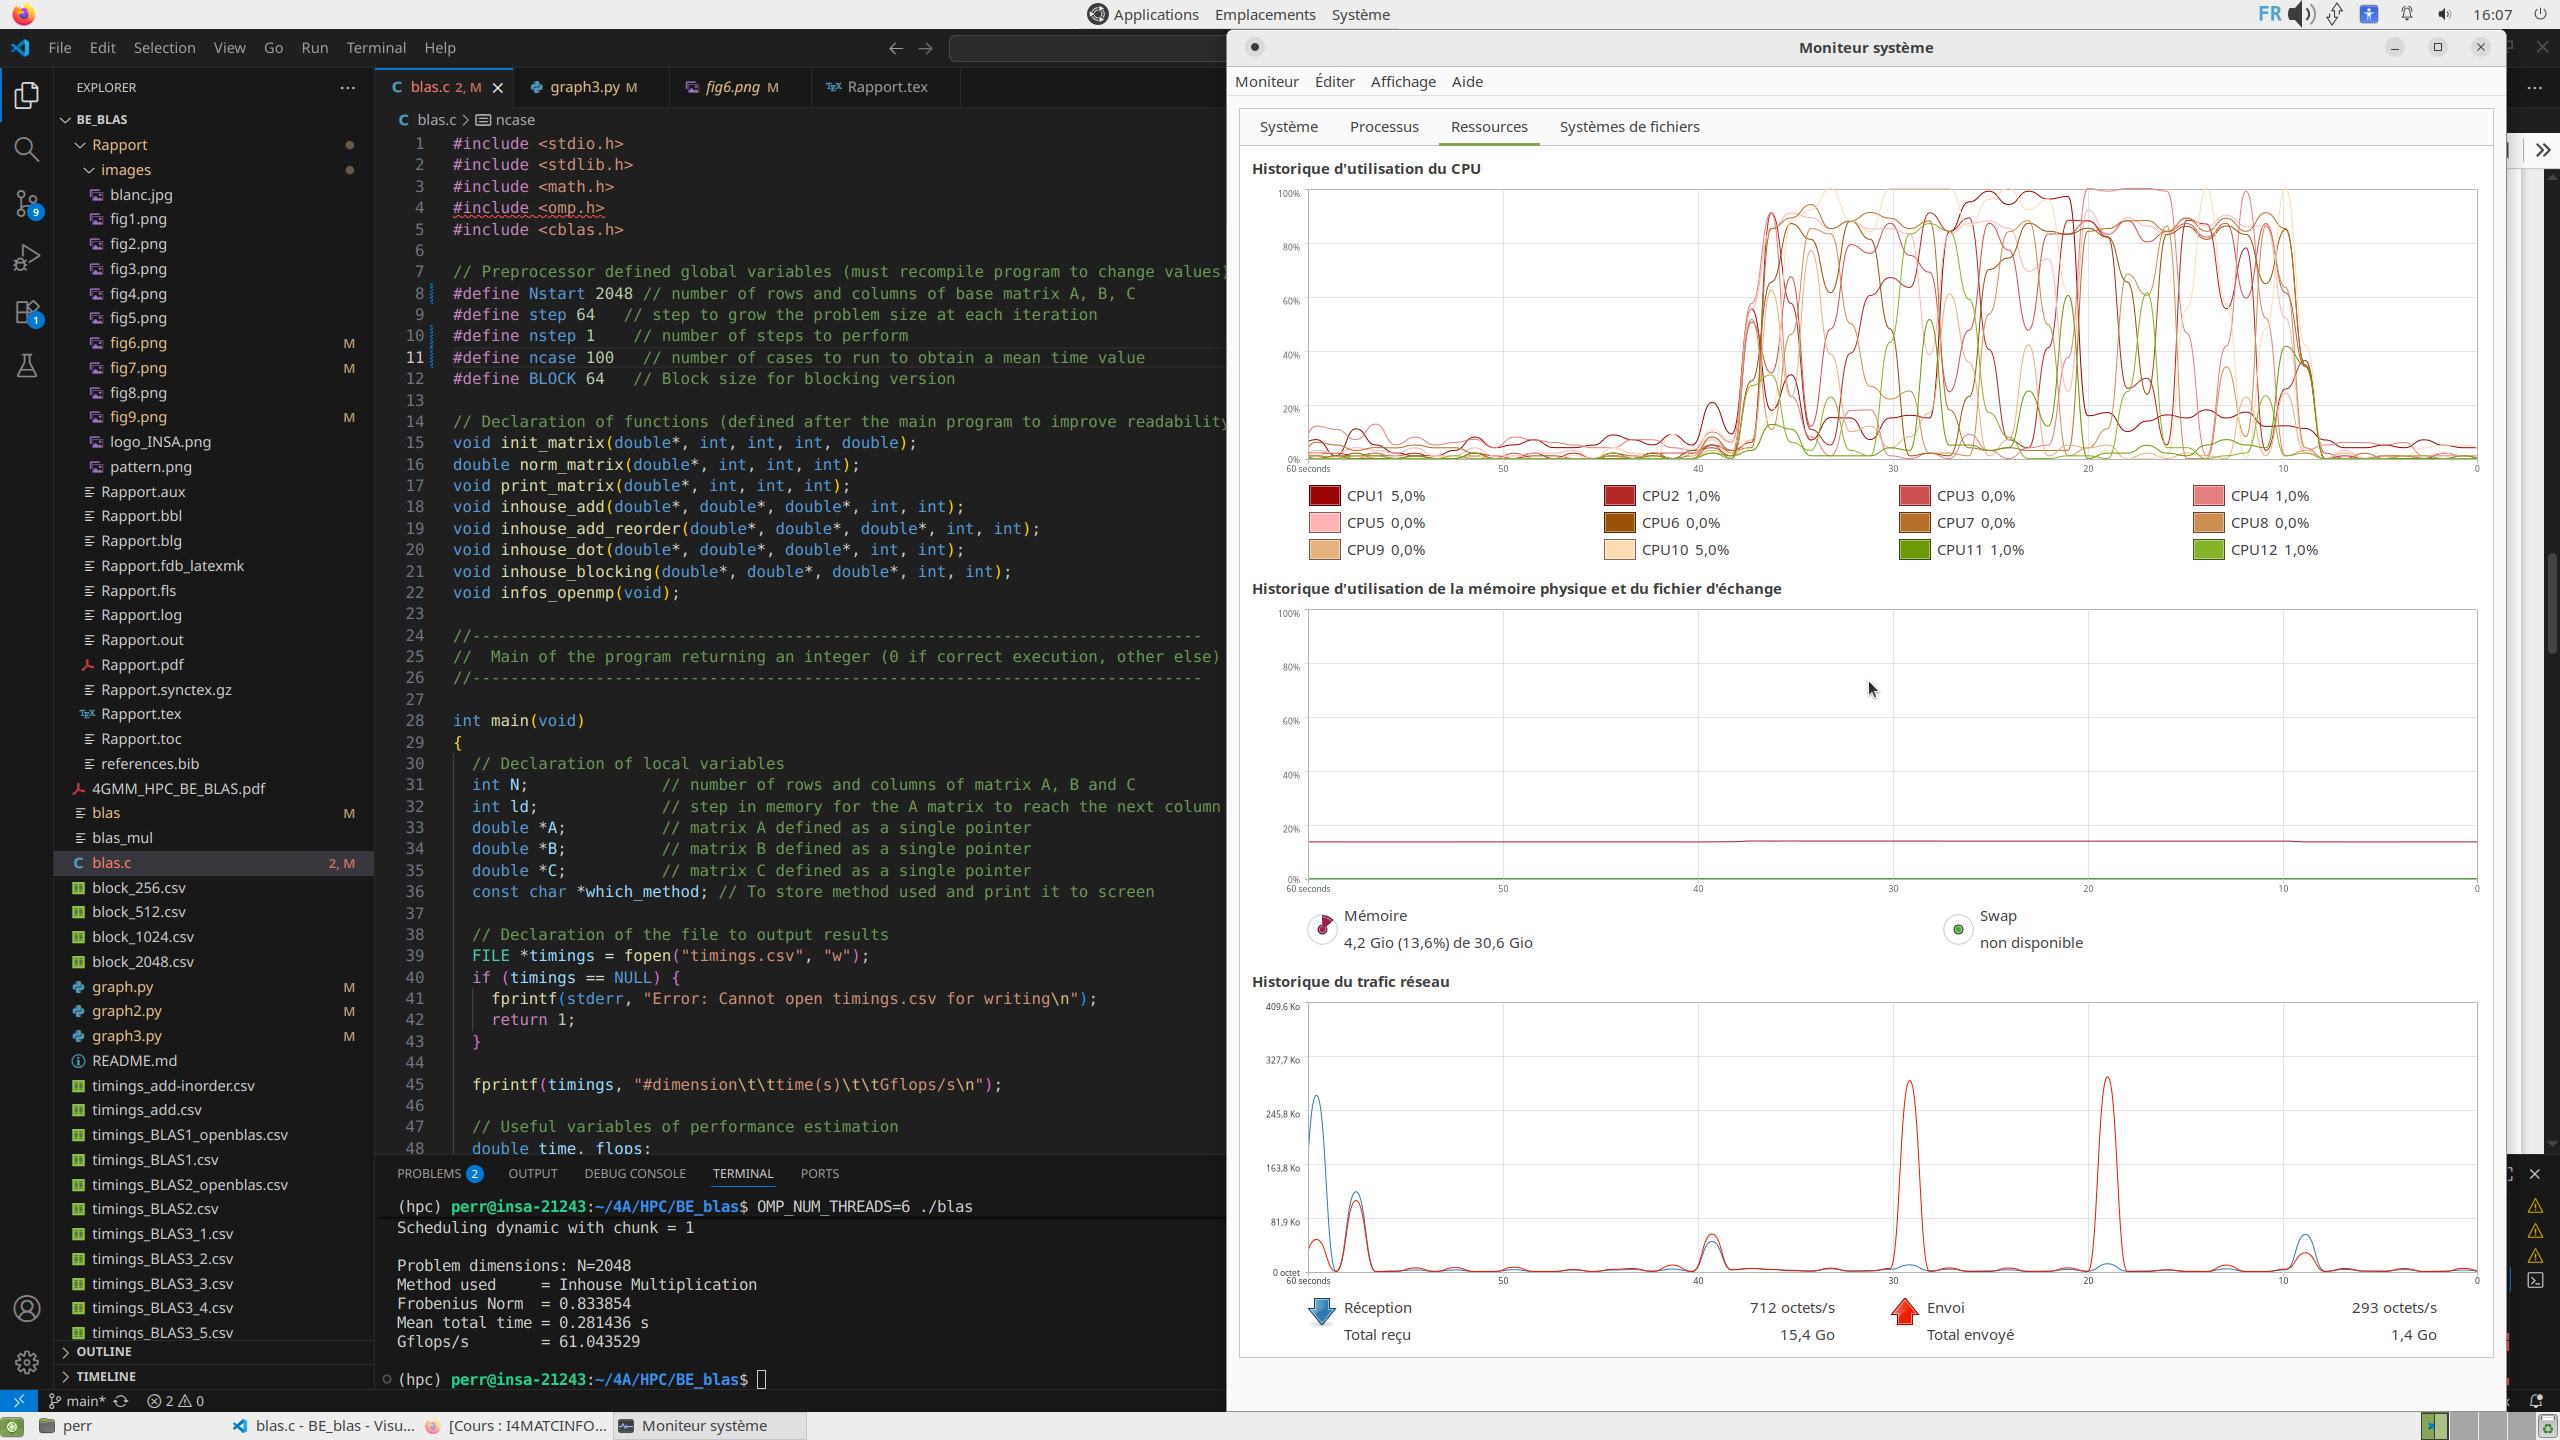
\includegraphics[width=0.7\linewidth]{images/useCPU.png}
    \caption{Trouver titre}
    \label{fig:7}
\end{figure}

Fait des tests de 1 à 12. Le nombre optimal c'est 6 parce que plus on parrallelise, plus on doit partager des données entre les différents threads. 

Expliquer que 6 threads qui ravail en permanence mais ce ne sont pas tout le temps les même.

\chapter{Utiliser les blocs du cache}

Expliquer la technique du block.

\begin{figure}[H]
    \centering
    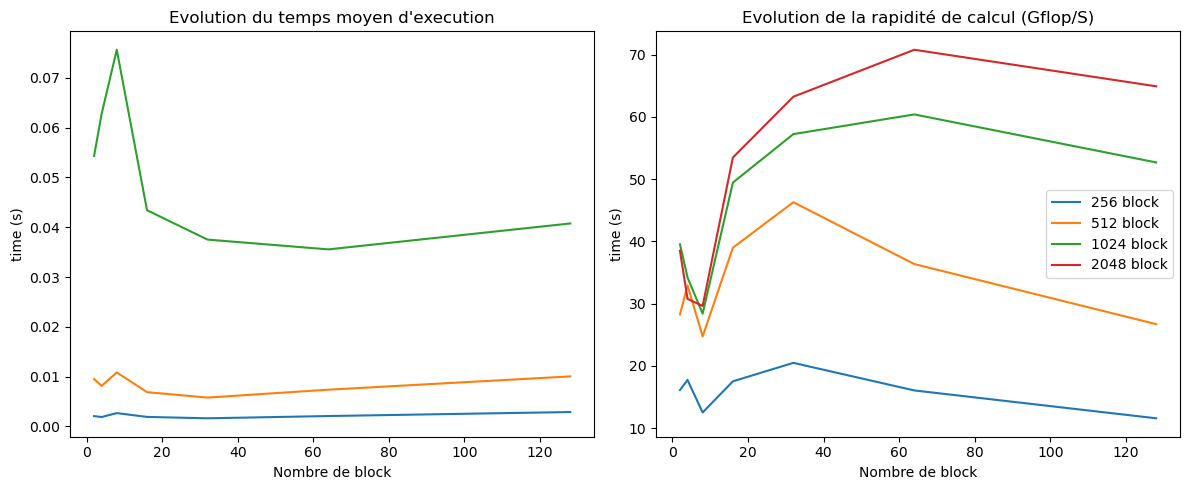
\includegraphics[width=0.7\linewidth]{images/fig7.png}
    \caption{Trouver titre}
    \label{fig:8}
\end{figure}

\begin{figure}[H]
    \centering
    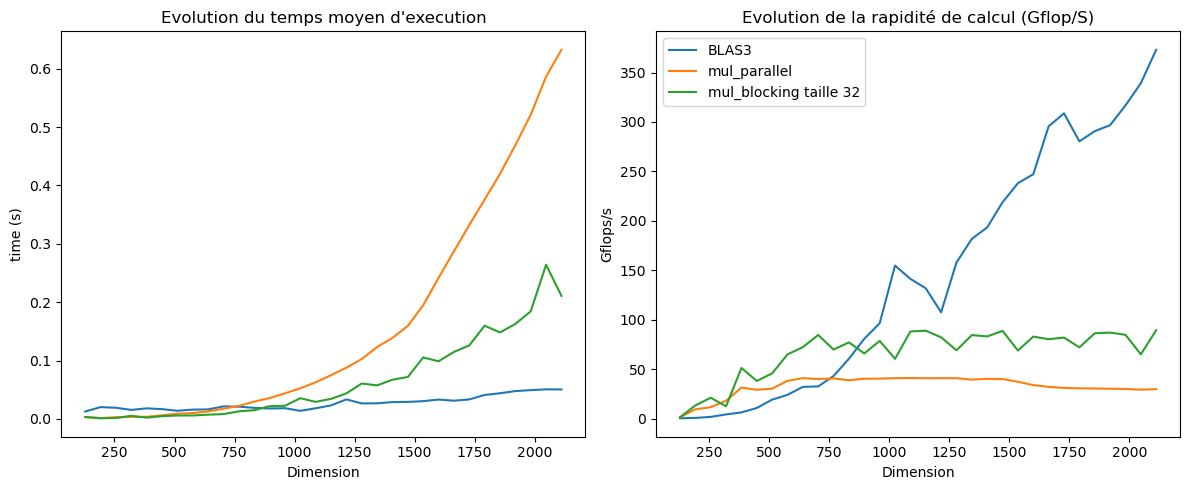
\includegraphics[width=0.7\linewidth]{images/fig9.png}
    \caption{Trouver titre}
    \label{fig:9}
\end{figure}

On a commencé par une rechercher de la taille de block optimale en fonction de différentes tailles de matrices. On a choisi 32 (mieux que 64).

Puis on a comparé cette technique avec openblas et la parralelisation.

On peut observer que la librairie openblas est la meilleure solution pour optimiser les performances de calcul en partageant efficassemet les thread.

\bibliographystyle{plain}
\bibliography{references}


\end{document}